\begin{solution}{hard} \textbf{a)} Let the height of the streamline flow far away from the wing to be $h_0$ and the height of the streamline flow at point $P$ to be $h_P$. Therefore, the continuity expression gives us:
$$u_0h_0=u_Ph_P \implies u_P=u_0\frac{h_0}{h_P}$$
here we are assuming that the airflow is completely two-dimensional, which means the area is proportional to the height. Note that we can only use this continuity expression with assumption (d) as the dynamic pressure is much smaller, which means effects caused by compression can be negligible. We can measure $h_0/h_P=0.77$ so we have $u_0=77 \text{ m/s}$. However, this is the speed of the air as measured by the plane. We can relate these quantities through:
$$\vec{v}_\text{air relative ground} = \vec{v}_\text{air relative plane} + \vec{v}_\text{plane relative ground}$$
Far away from the plane, $\vec{v}_\text{air relative ground}=0$ (no wind) so then the airplane must be travelling at a speed of $u_0$. Therefore, the speed of the air at $P$ relative to the ground is:
$$u_0-u_0\left(\frac{h_0}{h_P}\right)=\boxed{23 \text{ m/s}}$$
\begin{center}
    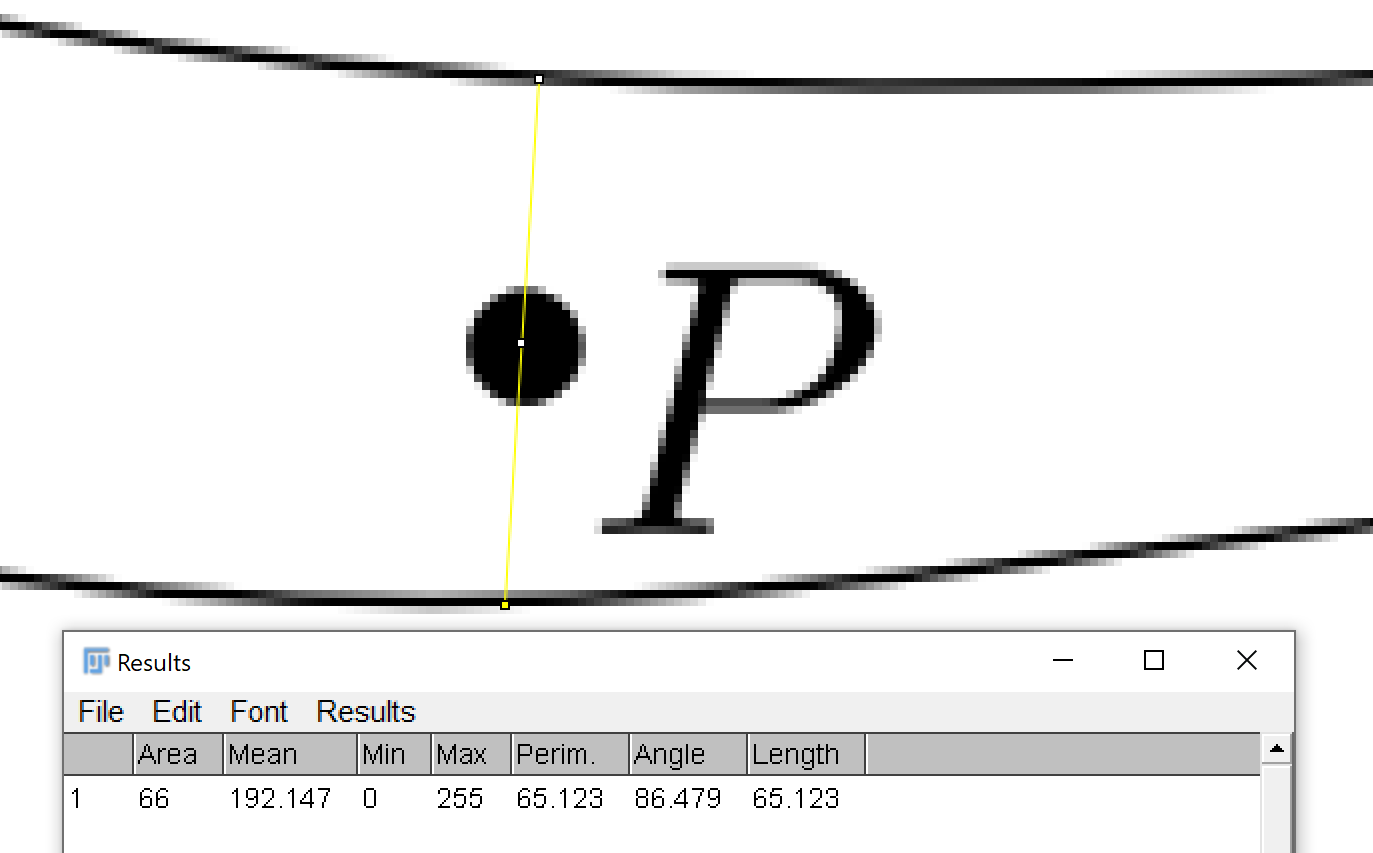
\includegraphics[width=12cm]{2012ipho1.png}
\end{center}
\begin{center}
    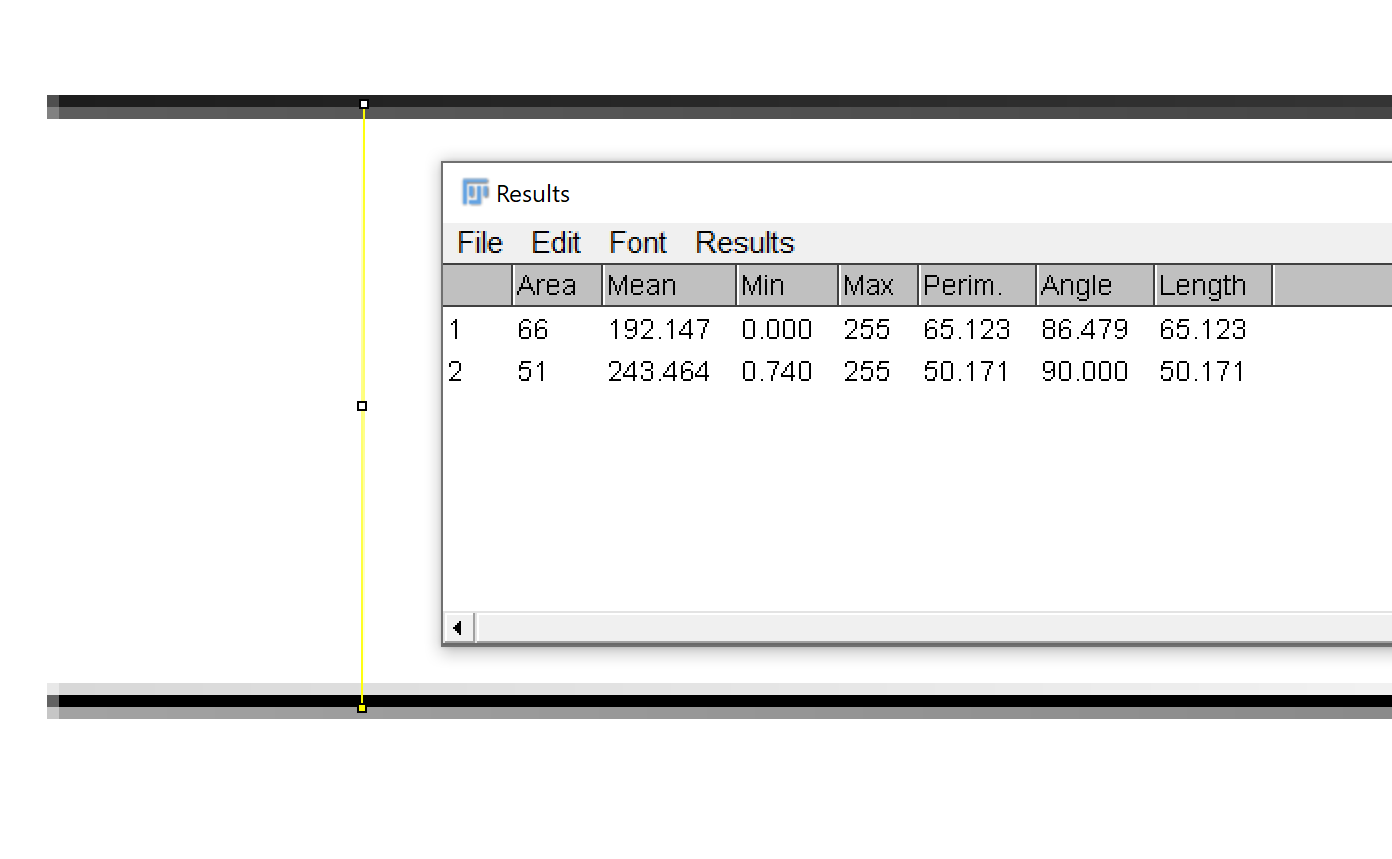
\includegraphics[width=12cm]{2012ipho2.png}
\end{center}
\vspace{3mm}

\noindent \textbf{b)} Using definition 10, condensation into water vapor is favored when the dynamic pressure $\frac{1}{2}\rho v^2$ is high. This occurs when $v$ is at a maximum, or when the streamline lines are close together. From the diagram, they are closest together at the top left corner of the wing.
\vspace{3mm}

\noindent \textbf{c)} From problem 17, we find that 
\[\frac{1}{2}v^2 + c_p T = 0.\]
We find from part a that,
\[\frac{1}{2}\Delta v^2 = \frac{1}{2}v_{\text{crit}}^2 \left(\frac{h_0^2}{h_Q^2} - 1\right) = c_p \Delta T\implies v_{\text{crit}} = \sqrt{\frac{2c_p\Delta T}{h_0^2/h_Q^2 - 1}}.\]
To finally solve this problem, we have to find $\Delta T$. By relating the ratios, we find that 
\[\frac{p_{\text{sa}} - p_{\text{w}}}{T_a - T} = \frac{p_{\text{sb}} - p_{\text{sa}}}{T_b - T_a}\implies T = \frac{p_{\text{sa}} - p_w}{p_{\text{sb}} - p_{\text{sa}}} (T_b - T_a) - T_a\]
where $p_w = rp_{\text{sa}}.$ We note that $\Delta T = T_a - T$, thus by substituting this into our final expression of $v_{\text{crit}}$, we find that 
\[v_{\text{crit}} = \boxed{\sqrt{\frac{2c_p}{h_0^2/h_Q^2 - 1}\left(\frac{p_{\text{sa}}(1 - r)}{p_{\text{sb}} - p_{\text{sa}}} (T_b - T_a)\right)}}.\]

\end{solution}